%%% Thesis Introduction --------------------------------------------------
\chapter{Introduction} \ifpdf
\graphicspath{{Introduction/IntroductionFigs/PNG/}{Introduction/IntroductionFigs/PDF/}{Introduction/IntroductionFigs/}}
\else
\graphicspath{{Introduction/IntroductionFigs/EPS/}{Introduction/IntroductionFigs/}}
\fi

Internet has become the predominant mode of communication in the modern
societies of our times. Currently, 1/3 of earth population is connected to the
Internet~\cite{itufacts2011}, while Internet-related business is estimated to
account for 3.4\% of the global GDP~\cite{duRausas:2011un}. In paraller, a large
fraction of our everyday social life requires network/Internet connectivity.
Regardless the vital role of computer networking in our life, its strong
backwards compatibility ties create a gap on our ability to evolve functionality
in order to fulfil current resource short-term requirements. As a result,
although the social setting requires novel functional properties from its global
network, it is rather difficult to provide it, without disconnect a portion of
it.

My work focuses on the evolvability problem of modern networks. The key idea of
this work focuses on ways to evolve computer network functionality through the
control plane. In this dissertation we argue the thesis that: 

\begin{quotation} Computer network should compat the problem of network
  ossification through context-aware evolved control planes, in order to provide
  new properties to their inter-connecting fabric. Such novel control plane
  implentations should focus on the requirements of the deployment environment
  and customly understand and fit their properties and functionalities. Such
  approach have to be deployed on the edges in order to obey the end-to-end
  principle.  \end{quotation}

For the remainder of this introduction we justify the importance of this thesis.
In section \ref{sec:intro:motivations} we present in details some of the
limitation that current Internet faces and the inherent limitations of current
architecture in terms of evolvability. In section \ref{sec:intro:contributions},
we list briefly the main contributions of this thesis and in section
\ref{sec:intro:outline}, we present briefly the content of each chapter of the
thesis. Finally, in section \ref{sec:intro:pubs} we list the publications
relating to the content of this thesis. 

\section{Motivation} \label{sec:intro:motivations}

\subsubsection*{Conputer network evolution}

\begin{figure}[ht] \centering \subfigure[global mobile traffic trend]{
    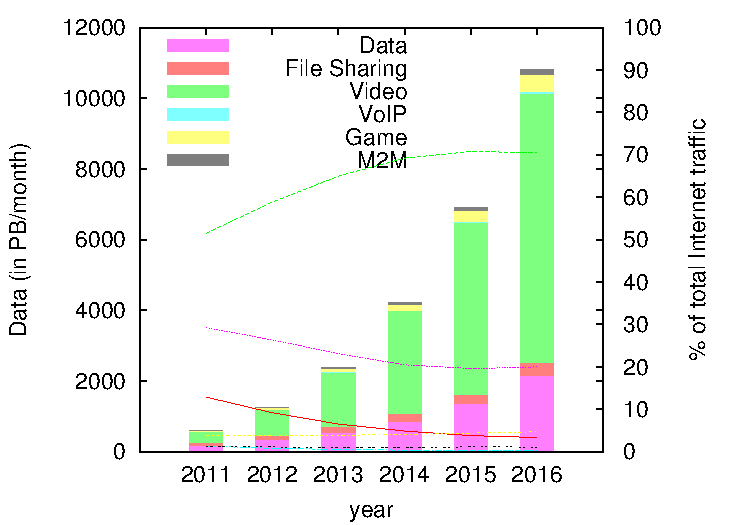
\includegraphics[width=0.45\textwidth]{mobile} \label{fig:internet} }
  \subfigure[global Internet traffic trend]{
    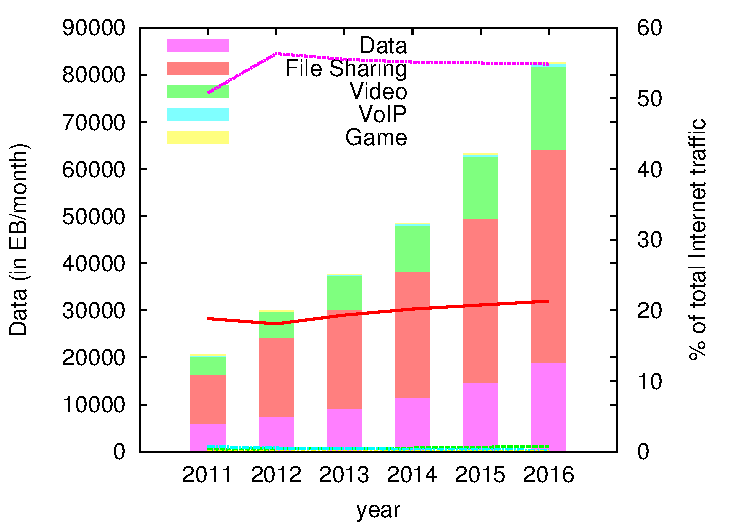
\includegraphics[width=0.45\textwidth]{internet} \label{fig:mobile} }
  \caption{Cisco Visual Network Index reports on global network traffic per
    application. Subfigure~\ref{fig:internet} provides details on the global
    Internet traffic trends, while Subfigure~\ref{fig:mobile} focuses on Mobile
    Internet traffic.} \label{fig:internet_applications} \end{figure}


\begin{table} \begin{center} \begin{tabular}{ | l | c c c c | } \hline
      Application  & rate & latency & jitter  & \# connections \\ \hline web
      & 0    & 0       & 0      & 0\\ video        & 0    & 0       & 0      &
      0\\ p2p          & 0    & 0       & 0      & 0\\ voip         & 0    & 0
      & 0      & 0\\ game         & 0    & 0       & 0      & 0\\ \hline
    \end{tabular} \end{center} \caption{Network performance requirement for a
    set of popular traffic classes.} \label{tbl:application_requirement}
\end{table}

% a historical prespective on computer networks 
One of the ideas that formed the subjective condition of the digital revolution
of our era, was the concept of computer networking. The initial goal of this
concept was to develop a new communication architecture that would allow
continuous communication over a redundant network, even when a significant
number of vertex was destroyed.  The main building block of computer networks is
the idea of packet-switched networks~\cite{Licklider1963}.  This idea gave birth
to the pioneer of today's Internet, the {\it ARPANET}~\cite{Mills:1987tt},
allowing for the first time in computing history communication between multiple
computers over a mess network. The initial set of applications that were
standardised where : e-mail~\cite{RFC0561}, ftp~\cite{RFC0354} and
voice~\cite{RFC0741}. This initial implementation was later replaced by the
NSFNET in the 80's, which finally devolved in today's Internet.
As part of this transition, the research community developed also the standards
for the TCP/IP protocol suite~\cite{Clark:1988}, the default protocol to provide
connectivity for the Internet.

% why computer networking is successful from the user perspective
Since the time of the ARPANET, computer networks have seen a significant
elevation on their role in the social apparatus of our world due to a number of
reasons. One of the most important trends, that boost their role, was the
radical reduction in cost, size and capabilities of network-enabled personal
computers, following Moore's Law model. The low cost factor of personal
computers along with the programmable nature of
the computer CPU, makes it an elegant platform to develop applications that
introduce seamlessly new functionalities. Nowadays, programmable CPUs are
integrated in a number of multi-purpose devices such as mobile phones, display
devices etc, while the ability of personal computers to transform in size,
introduces new computing concepts, such as laptops, tablets and other.
As a result, the paradigm of one computer per household of the 90's rapidly
shifted to the paradigm of multiple devices per user, replacing a number of
everyday single-purpose devices~\cite{Dholakia:2006vn}.  On one hand, this
augmentation in computational devices requires new modes of communication that
allow devices to share consistently state, driving a significant development in
computer network technologies. A number of network-enabled applications are
developed to address these requirements, while new network paradigms are
introduced like home networks and hotspots. Existing computer network
technologies make this work easy, as they only require a minimal implementation
of a protocol and a peer with a forwarding entity in order to establish
connectivity with any other device. On the other hand, the elevated role
of computer networks and the introduction of the cloud computing paradigm,
introduce a number of internet-wide services with a global scope. 
% These new
% applications introduce a number of new assumptions on performance and
% connectivity over the Internet abstraction.  
The important role of computer
networks can be further reflected in the government level debate to proclaim
Internet connectivity as a fundamental human right~\cite{klang2005human}.

% why computer become important for the global economy too? 
In parallel with the development of the personal computer paradigm, computer
network are widely adopted as an integral asset for industry.  Currently the
Internet produces 4,3\% of the global GDP. Computer Networking and the Internet,
provide the middleware to interconnect modern multinational businesses. In the
business domain computer network have become popular and important for two main
reasons: computer networks provide a cheap and fast communication medium
to interconnect the business logic, and distribute
content to users. The adaptation of computer network has further augmented
through the utilisation of the cloud as a medium to offload infrastructures to
3rd party cloud providers, reducing to a great extend the cost of running
services in house.\todo{add a reference to the value of the cloud industry.}

% what about the application requirements 
The wide adaptation of computer networks has introduce a number of new use cases
and applications. Computer networking depends to a great extend on the
abstraction design pattern in order to support scalability and heterogeneity.
The abstraction principle is based to a great extend on the OSI
model~\ref{Day:1983vy}, which tries to separate network functionality into a
number of layers and define the interface provided by each layer. A side effect
of this design is that application developers don't have access on the
properties of the underlying path.  The OSI model or
the TCP/IP implementations provide semantics for the interfaces but they don't
provide any guarantees on the performance properties.  Applications on the other
hand, have performance requirement which they try to 'enforce' in the deployed
environment. As a result, resource allocation in a network becomes difficult due
to the diverse nature of network applications. In order to exemplify the problem, 
we list in Table~\ref{tbl:application_requirement} a number of key traffic properties 
for popular traffic classes of the Internet. Network applications have
diverse properties which becomes difficult to address during network congestion. 

% How computer application mix looks in the wire? 
Network planning for long term periods is also difficult to address.  The main
cause of this problem is the high churn in the  popularity of network
applications.  In order to exhibit this trend, we plot in
Figure~\ref{fig:internet_apllications} the global prediction on traffic volumes
for popular application classes for five years. We use data from cisco
visualization index white papers~\cite{Mobile:2012vd,Cisco:2012wu}. In the
histogram we can see that network traffic is expected to increase an order of
magnitude for the mobile environment, while the global Internet traffic is
expected to increase four times. In parallel, application volumes evolve
unevenly between traffic classes. File sharing services are expected to reduce
their share of the total volume, replaced by web and video delivery services. 

% How does the network look like in terms of point to point connectivity. 
High diversity is also observed on the properties of available mediums for
computer networks. The properties of links is defined in the data link and
physical layer of the OSI model. Currently, Ethernet is the predominant link
layer protocol in the Internet. In the 80s the low cost property of Ethernet
implementations establish it as the leader of the market ever since.  The
protocol has developed standards to run over coper and optical mediums, as well
as off-licence radio frequencies, satellite and mobile networks. Although the
Ethernet abstraction is persistent among all these mediums, it hides a lot of
the performance limitations of the link (e.g. packet loss, hop-by-hop ARQ etc.).
Because of this diversity in links, the performance of a computer network can be
variable. An example of this property is the Internet. Internet exhibits a 3
layer hierarchy of ASes, which allows it to scale and provide short-length paths
between any 2 nodes.  Tier 1 and 2 ISPs provide forwarding in an homogeneous and
fast manner. Such ISP's are in charge of a relatively small number of network
points and thus are able to upgrade network infrastructure with relatively low costs,
which can further be offloaded to clients through SLA agreements. For Tier-3 ISPs things
are a lot different. This class of ISPs covers a wide range of services. Also
because this is the last hop to end users, such networks tend to be large and
spread over large geographic distances. For this type of networks, connectivity
properties are variable, users SLA have minimum guarantees, performance can be
highly dependent on link sharing ratio and can be highly variant
due to the heterogeneity of medium types. Additionally, the cost to upgrade such
networks is high, while strong market competition makes difficult to offload
costs directly to users. A number of measurement studies have
described these differences~\cite{Huang:2010wb,Dischinger:2007bg}. 

\subsubsection{Computer network ossification}

% how does computer networks look like, How the Internet looks like?
% Over the previous section we described the heterogeneity of current computer
% networks and the dynamics of network applications. In order to address these
% properties in an efficient way, computer network technologies should be able to
% evolve. But within existing network systems it is difficult to deploy new
% technologies. 
Although computer networks are highly important for society the adaptability of
network technologies to user requirement has not been equal over the years. This
mismatch can be ascribed to a number of reasons. 

% network design were developed in an environment that had different properties
Current network technologies were developed a number of years ago in order to
develop standardized and generic mechanisms to interconnect
research institutes. Although DARPA funded the idea of computer networks in
order to develop new resilient communication mechanisms, the early adopters of
the technologies were universities and research facilities. As a result,
protocols were developed by computer scientist taking under consideration the
properties of such environments. The TCP/IP protocol suite was develop during
the transition of the ARPANET to NSFNET. Since then, the TCP/IP protocol suite
has been the default standard of the Internet.  During the first period of the
NSFNET, a number of competitive suites were developed which addressed in their
specification the problem of extensibility~\todo{find references for OSI TP*
  protocol and ATM UNI}.  Unfortunately, the increased design complexity made it
difficult to develop high performance implementations, and they soon
were declared obsolete by the network community. The TCP/IP protocol suite provided a fair
split between simplicity and extensibility at that time.

Nontheless, in the recent years the limitations of TCP/IP abstraction have
become apparent, as a number of fundamental assumptions has changed. Some of the
core limitations of the protocol can be described in the following points:

% Why current abstraction is not sufficient to fulfil network requirements. 
% Some assumption are invalid, while other assumption have been dropped by
% design. 
% Introduce the reason behind protocol ossification and computer network
% evolution limitations 
% Some concrete examples of how computer networks are insufficient 
\subparagraph*{Elevated Role of Security}: 
An important architectural goal for the design of computer network was the
minimization of functional requirements from joining hosts, allowing wide
adoption of the technology and open accessibility.  When the idea of computer
networks was first developed, the capabilities of computer hardware were limited
and network connectivity should not consuming a significant portion of the
computational resources of a node. As a result, the initial security
requirements from computer network technologies were minimal. In the recent
years, due to the vital role of computer networks in industry, security
requirements expanded. A McAfee report from 2009 reports that the cost of
cybersecurity is calculated to approximately six hundred million
dollars~\cite{Acherman:2009wf}. The threat model lurcking over the Internet is
wide and contains a number of threats, from Information interception to
denial-of-service attacks. Such costs can be reduced to a great extend if the security
was inherent to network protocols, span from the lowest levels of the
network abstraction and spread across the network. Attempts to address such
problem have been proposed in the protocol community, e.g. IPSEC~\cite{RFC2401},
but the deployment at the moment is not straighforward.

\subparagraph*{Network Addressing}: When the IP protocol was firstly deployed in
the Internet, the size of the network was sufficiently small. Addressing was
assigned based on a 32-bit integer space, split in byte aligned classes in order to permit
aggregation at the forwarding entities. Within 10 years, the initial assumption
over the size of classes was re-established through the classless Inter-domain
routing (CIDR), in order to allow better utilisation of the IP space. Within 15
years  though the initial assumption over the size of the address space prooved
also shortviewed, as IP addresses were not sufficient to cover the needs of hosts.
A number of layer violations, like NATs, were widely used within the subsequent
years in order to provide connectivity to the increasing number of end-hosts. In
order to address this problem within the design of the network protocol, a
revised version of IP has been proposed~\cite{RFC2460} since 1998, but its
deployment is slow, as the size of the current Internet makes it extremely
difficult to replace IPv4 without significant connectivity problems and costs.

\subparagraph*{Resource allocation}: Internet provides 
a best-effort forwarding mechanism. This design decision was chosen in order to
enforce the end-to-end principle of the Internet~\cite{end2endIP} and avoid
state in the intermediate nodes of the network. Such an approach covered 
sufficiently the requirements of the networked applications of the time. As new
network application became available over the years, more strict performance
requirements were introduced. Unfortunately, Internet currently has no mechanism 
to address these requirement network-wide. Network engineers have tackled this
problem through adequate resource provision~\cite{TeiSha02}. This approach
though becomes inefficient as network rates increase. In a 40gbps link the impact
of queueing delays or packet drop becomes significant to the performance of streams.
In related literature, a number of approaches has been proposed to address this
problem in multiple layers of
the network stack~\cite{RFC5562, RFC2475, RFC3135}. Unfortunately, such
approaches are
difficult to deploy across large networks, as they require significant upgrade
in network elements, introducing a significant cost. 

\subparagraph*{Bidirectional connectivity}: A side-effect of mechanisms
addressing the previous two problem is the collapse of a fundamental assumption
of computer network design, the ability of two connected nodes to communicate. A
node which is behind a traffic inspecting middlebox is not guaranteed 
to receive incoming connections from any node and thus is not
fully interactive. This problem has a direct consequence for users to resolve
to 3rd party services in order to establish connectivity, changing as a result
the communication mechanism. 

% discussion on ossification. Why evolution on protocol is difficult?
A number of problems that we experience with current network functionality can
be traced back to the assumptions of the protocols. A number of clean slate
approach have been proposed over the years, that address a number of these
problems. The process though to deploy a new protocol is not straightforward.
Computer networks currently suffer from an effect that is term as \{it 'protocol
  ossification'\} in the research community. The protocol hierarchy in the
internet currently looks like an hourglass. We currently have a multitude of
protocol in the application and link layer, but we only have IP in the network
layer and TCP and UDP in the transport layer. The specifications of these
protocol define a number of mechanisms that allow protocol designers to develop
extensions.  Unfortunately, these mechanisms are not guaranteed to be supported
across the network, as their support is not critical for functionality and thus
can be sacrifices in favour of performance. As a result, the capabilities to
evolve protocol in a manner that is compatible with the current Internet
infrastructure is impossible. In~\cite{Bauer:2011ws} authors report that 80\% of
popular services doesn't support ECN and 0,6\% of destination may drop ECN
traffic, while in~\cite{Honda:2011ci} authors report a large scale inability of
the Internet to cope with TCP traffic that carries unknown option fields. 

% wrap-up - Things are tricky. 


\section{Contributions} \label{sec:intro:contributions}

\section{Outline} \label{sec:intro:outline}

\section{Publications} \label{sec:intro:pubs}
As part of my PhD work the following work was published by me:
\begin{itemize}
  \item Rotsos, C., Van Gael, J., Moore, A. W., \& Ghahramani, Z. (2010).
        Probabilistic graphical models for semi-supervised traffic
        classification (pp. 752–757). Presented at the IWCMC '10: Proceedings of
        the 6th International Wireless Communications and Mobile Computing
        Conference.
  \item Mortier, R., Ben Bedwell, Glover, K., Lodge, T., Rodden, T., Rotsos, C.,
        et al. (2011). Supporting novel home network management interfaces with
        openflow and NOX. Presented at the SIGCOMM '11: Proceedings of the ACM
        SIGCOMM 2011 conference,  ACM. doi:10.1145/2018436.2018523
  \item Madhavapeddy, A., Mortier, R., Gazagnaire, T., Proust, R., Scott, D.,
        Singh, B., et al. (2011). Constructing a “Functional” Cloud (Mirage
        2011), 1–10.
  \item Mortier, R., Rodden, T., Lodge, T., McAuley, D., Rotsos, C., Moore, A.
        W., et al. (2012). Control and understanding: Owning your home network
        (pp. 1–10). doi:10.1109/COMSNETS.2012.6151322
  \item Rotsos, C., Sarrar, N., Uhlig, S., Sherwood, R., \& Moore, A. (2012).
        Oflops: An open framework for openflow switch evaluation, 85–95.
  \item Chaudhry, A., Madhavapeddy, A., Rotsos, C., Mortier, R., Aucinas, A.,
        Crowcroft, J., et al. (2012). Signposts: end-to-end networking in a
        world of middleboxes. Presented at the SIGCOMM '12: Proceedings of the
        ACM SIGCOMM 2012 conference on Applications, technologies,
        architectures, and protocols for computer communication,  ACM.
  \item Rotsos, C., Mortier, R., Madhavapeddy, A., Singh, B., \& Moore, A. W. C.
        I. 2. I. I. C. O. (n.d.). Cost, performance \& flexibility in OpenFlow:
        Pick three. Presented at the Communications (ICC), 2012 IEEE
        International Conference on.
  \item Madhavapeddy, A., Mortier, R., Rotsos, C., Scott, D., Singh, B.,
        Gazagnaire, T., et al. (2013). Unikernels: Library Operating Systems for
        the Cloud. Proceedings of ASPLOS.  
\end{itemize}



% Todays Internet depends to a great extend on protocols and systems designed by
% its creators from the 70's. The requirement for wide heterogeneity and
% backwards compatibility reduces our ability to innovate and evolve current
% network systems. In parrallel though, computer networks are currently a
% significant asset for the development of humanity, a state which imposes a set
% of multi-functional requirements over their deployment. The thesis of this
% dissertation is : \begin{quote} Modern computer networks can enhance their
% ability to provide better user experience through control plane evolution. By
% enhancing the control plane of an SDN architecture with user requirement, we
% can enable optimal resource allocation.  \end{quote}
% 
% \begin{quotation} In the recent years, the Internet has met an incredible
% development in terms of infrastructure as well as connectivity. This
% development has been driven by two main causes: the significant reduction of
% the cost of network-enabled device and the subsequent widespread adoption from
% users and the wider utilization from companies of the Internet as a medium to
% interconnect and expand their market. Although significant, Internet
% development has been highly asymetric. The capacity of the core of the
% Internet has increased exponentially over the recent years and routing has
% become stable.  As a result, the network bottleneck has moved to the edges of
% the Internet, a point where link upgrades have a significantly higher
% aggregate cost and access technologies have seen little innovation.  In this
% work, I argue that edge networks performance is further reduce due to a great
% extend to the way many internet scale protocols are deployed.  Further, I
% believe that in order to handle more efficiently resources in the edges,
% functionality of network devices should be customized to the needs of the
% specific environment and network processing should be developed over newer
% abstractions, that match the flow primitives of the specific environment. In
% this work I focus in the case of home networking and I present a number of
% novel network designs that leverage the ability to control and use home
% networks.  \end{quotation}

% In the introduction I think it is important to mention the following points: %
% I am planning to present 2 main points: \begin{itemize}
% \item The core of the Internet is highly optimized and can perform really well
%       the task of packet forwarding end-to-end. Although the programmability
%       of the core is restricted due to the low cost principle and the high
%       multiplexing of network connections. On the other hand, edge networks
%       exhibit lower connection multiplexing which make programmability 
% to be handle using restricted resources. Further, in the edges we are able to
% integrate in the packet processing process useful input from the users. There
% a number of measurement studies that present this differentiation both for the
% ADSL/cable (Netanalyzer, bufferbloat, ADSL measurement studies) world, as well
% as 3g (e.g. 3gtest).
% \item The concept of network programmability is not a new concept. It has
%       already been discussed in different forms (e.g. ATM
%       controllers/switchlets, active networks) which though never manage to
%       get deployed in the real world. I need to discuss for the most
%       significant cases, why these mechanisms failed to meet their
% requirements and why the SDN approach solves some of their problems. 
% \item An additional problem that I should discuss in this chapter is the
%       different abstractions perceived by network applications and service
%       providers. This difference in abstractions result in a significant loss
%       of information that could potentially be used by both sides in order to
%       optimize
% network utilisation.
%
% \end{itemize}
%%% ----------------------------------------------------------------------
%%% Local Variables: 
%%% mode: latex
%%% TeX-master: "../thesis"
%%% End: 
